\section{将按分组PRF转化为按比特PRF}\label{sec:6-8}

到目前为止,我们为 $\mathcal{X}^{\leq\ell}$ 上的变长输入构建了一些 PRF。通常 $\mathcal{X}=\{0,1\}^n$,其中 $n$ 是底层 PRF 的分组大小,CBC 或者级联构造都基于该参数构建(例如,对于 AES,$n=128$)。迄今为止,我们所介绍的所有 MAC 都被设计用来验证长度为 $n$ 比特的倍数的消息。

在本节中,我们将展示如何将这些 PRF 转换为针对任意长度消息的 PRF。也就是说,给定一个针对 $\mathcal{X}^{\leq\ell}$ 上的消息的 PRF,我们想要构建一个针对 $\{0,1\}^{\leq n\ell}$ 上的消息的 PRF。

令 $F$ 是一个接受 $\mathcal{X}^{\leq l+1}$ 中输入的 PRF。令 $inj:\{0,1\}^{\leq n\ell}\to\mathcal{X}^{\leq\ell+1}$ 是一个单射(即一对一)函数。定义派生出的 PRF $F_{\rm bit}$ 为:
\[
F_{\rm bit}(k,x):=F(k,\,inj(x))
\]
于是,我们可以得到下面的一个三段式定理。

\begin{theorem}\label{theo:6-10}
如果 $F$ 是一个定义在 $(\mathcal{K},\mathcal{X}^{\leq\ell+1},\mathcal{Y})$ 上的安全的 PRF,则 $F_{\rm bit}$ 是一个定义在 $(\mathcal{K},\{0,1\}^{\leq n\ell},\mathcal{Y})$ 上的安全的 PRF。
\end{theorem}

\begin{figure}
  \centering
  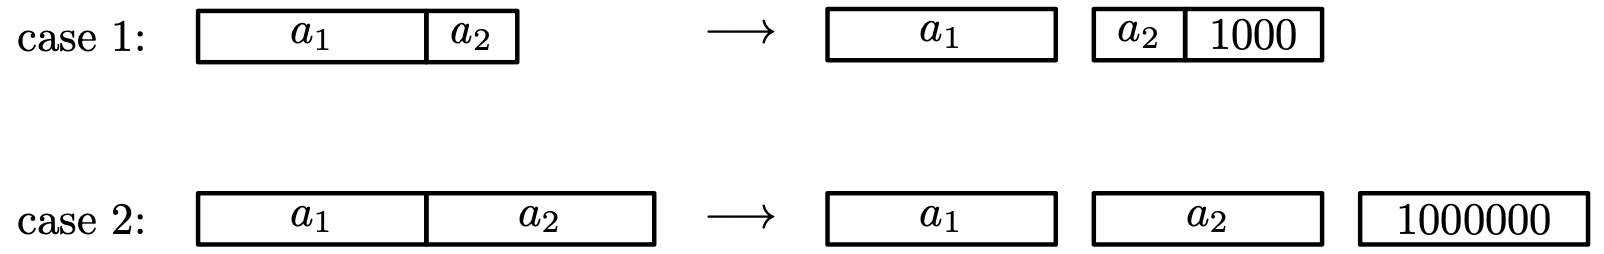
\includegraphics[width=0.75\linewidth]{figures/chapter6/fig7.png}
  \caption{一个单射函数 $inj:\{0,1\}^{\leq n\ell}\to\mathcal{X}^{\leq\ell+1}$}
  \label{fig:6-7}
\end{figure}

\begin{snote}[一个单射函数。]
对于 $\mathcal{X}:=\{0,1\}^n$,一个从 $\{0,1\}^{\leq n\ell}$ 到 $\mathcal{X}^{\leq\ell+1}$ 的单射 $inj$ 的标准例子如下。如果输入消息的长度不是 $n$ 的倍数,那么 $inj$ 会添加 $100\dots00$ 来填充消息,使得它的长度成为 $n$ 的倍数,图 \ref{fig:6-7} 以图像的形式直观地刻画了这一点。更准确地说,该函数的工作原理如下:

\vspace{5pt}

\hspace*{5pt} 输入:$m\in\{0,1\}^{\leq nl}$

\vspace{3pt}

\hspace*{5pt} 令 $u\leftarrow|m|\;\mathrm{mod}\;n$,$m'\leftarrow m\,\Vert\,1\,\Vert\,0^{n-u-1}$\\
\hspace*{26pt} 输出 $m'$ 作为 $n$ 比特消息分组的一个序列

\vspace{5pt}

\noindent
为了说明 $inj$ 是一个单射,我们先表明它是可逆的。给定 $y\leftarrow inj(m)$,从右到左扫描 $y$,并删除所有 $0$ 和初次见到的 $1$,那么剩下的序列就是 $m$。

\vspace{5pt}

一个常见的错误就是用一个全 $0$ 的填充序列将给定的消息填充成分组长度的倍数。这样的映射并不是单射,并且会产生一个不安全的 MAC:对于任何长度不是分组长度的整数倍的消息 $m$,其 MAC 也是 $m\,\Vert\,0$ 的一个有效 MAC。因此,这样的 MAC 容易受到存在性伪造攻击。
\end{snote}

\begin{snote}[单射函数必会扩充。]
当我们把一个 $n$ 比特的单分组消息输入 $inj$ 时,该函数必须要增加一个``假"分组,并输出一个两分组消息。这对于那些主要以单分组消息为对象的应用来说是很不利的。当使用 CBC 或级联构造时,假分组迫使签名者和验证者对于每条消息都要评估两次底层的 PRF,就算所有的消息本身都只有一个分组。结果就是,所有参与方的计算量都被翻倍了。

因此,我们很自然地想要找到一个不需要添加假分组的单射函数。但不幸的是,这样的函数是不存在的,因为集合 $\{0,1\}^{\leq n\ell}$ 比集合 $\mathcal{X}^{\leq\ell}$ 要大。因此,所有的单射函数都必须要在输出中添加一个``假"分组。

我们将在 \ref{sec:6-10} 节介绍的 CMAC 构造为这个问题提供了一个优雅的解决方案。CMAC 通过使用一个\emph{随机化的}单射函数来避免添加假分组。
\end{snote}